\documentclass[titlepage,letterpaper,12pt]{article}
% Plantilla para trabajos escolares

\usepackage[T1]{fontenc}
\usepackage[utf8]{inputenc}
\usepackage[spanish]{babel}
%\usepackage[margin=.5in]{geometry} % márgenes
\usepackage{graphicx} % para las imagenes
\usepackage{subcaption}
\usepackage{wrapfig}
\graphicspath{ {./img/} }
%\usepackage{xcolor} % para los diagramas uml
%\usepackage{tikz}
\usepackage{enumitem} % para las listas de definicion
\usepackage{mathptmx} % para Times
\usepackage{minted}% para código
\usemintedstyle{vs}
\fontfamily{ptm}\selectfont
\AddToHook{cmd/section/before}{\clearpage}

% titulo, autor, fecha, equipo
\newcommand{\portadae}[5]{
  \begin{titlepage}
    \begin{center}
      \Huge
      Universidad Nacional Autónoma de México

      \vspace*{1cm}

      \LARGE
      Facultad de Ingeniería

      \vspace*{1cm}

      \Large
      Programación orientada a objetos

      \vspace*{1cm}

      \large
      Prof. Edgar Tista García

      \vfill

      \LARGE
      \textbf{#1}

      \vfill

      \Large
      Equipo #4

      \vspace*{1cm}

      \textbf{Integrantes:}

      #2

      \vfill

      %\includegraphics[width=0.4\textwidth]{university}

      \textbf{Fecha de entrega}

      #3
    \end{center}
  \end{titlepage}
}

\usepackage{emoji}

\begin{document}
\portadae{Manual de usuario para máquina de casino}{Garciliano Díaz Giovanni Alfredo}{31 de mayo de 2022}{2}

\tableofcontents

\section{Prólogo}
El siguiente documento describe todas las acciones que se pueden realizar con este programa. Se presentan dos puntos de vista, según los dos tipos de usuario que existen en el programa: jugadores y administradores. Un perfil de jugador puede realizar las operaciones normales para las que fue diseñado el programa: jugar, apostar, y agregar dinero al sistema. Por otra parte, los perfiles de administrador no están pensados para jugar: éstos permiten modificar otros usuarios, crear y eliminar nuevos, pero no permiten jugar. Entonces, un administrador que desee jugar deberá tener dos cuentas: una de administrador para realizar sus tareas administrativas, y una de usuario para sus tareas lúdicas. En este manual encontrará cada tipo de actividad en una sección distinta, por lo que se exhorta al lector leer completamente este manual antes de ejecutar el programa por primera vez.

Adicionalmente, se ha incluido un pequeño glosario en la última sección de este documento, con el fin de aclarar al lector los significados de algunos términos técnicos cuyo significado pudiera ser desconocido para el mismo.

\subsection{JRE}
Ahora bien, antes de poder ejecutar el juego, es necesario verificar que se tenga instalado, como mínimo, la versión 8 de Java Runtime Environment, que puede obtenerse desde el sitio web oficial de Oracle\footnote{https://www.oracle.com/java/technologies/downloads/}. Si se desea obtener una versión completamente libre del Java Development Kit, puede obtenerse desde el sitio oficial del proyecto OpenJDK\footnote{https://jdk.java.net/java-se-ri/8-MR3}, bajo la licencia GNU GPLv2. Esto funciona para los sistemas Windows.

\begin{figure}[h]
  \centering
  \begin{subfigure}[b]{.5\textwidth}
    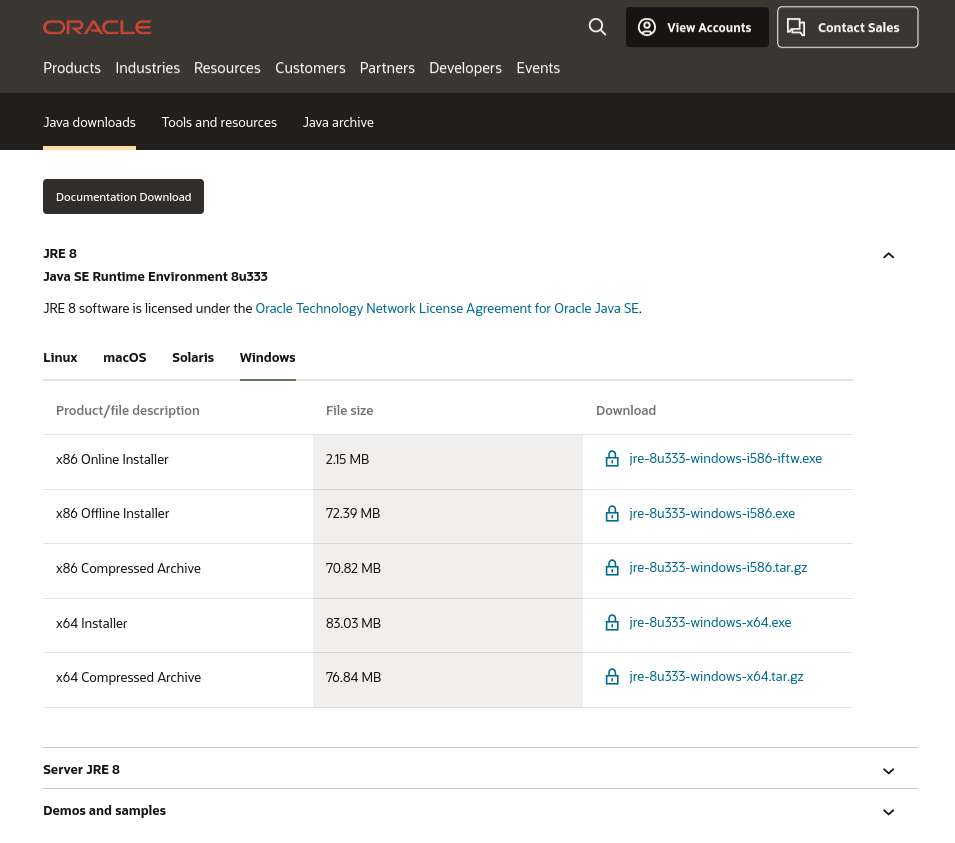
\includegraphics[height=6cm]{manual01}
  \end{subfigure}
  ~
  \begin{subfigure}[b]{.3\textwidth}
    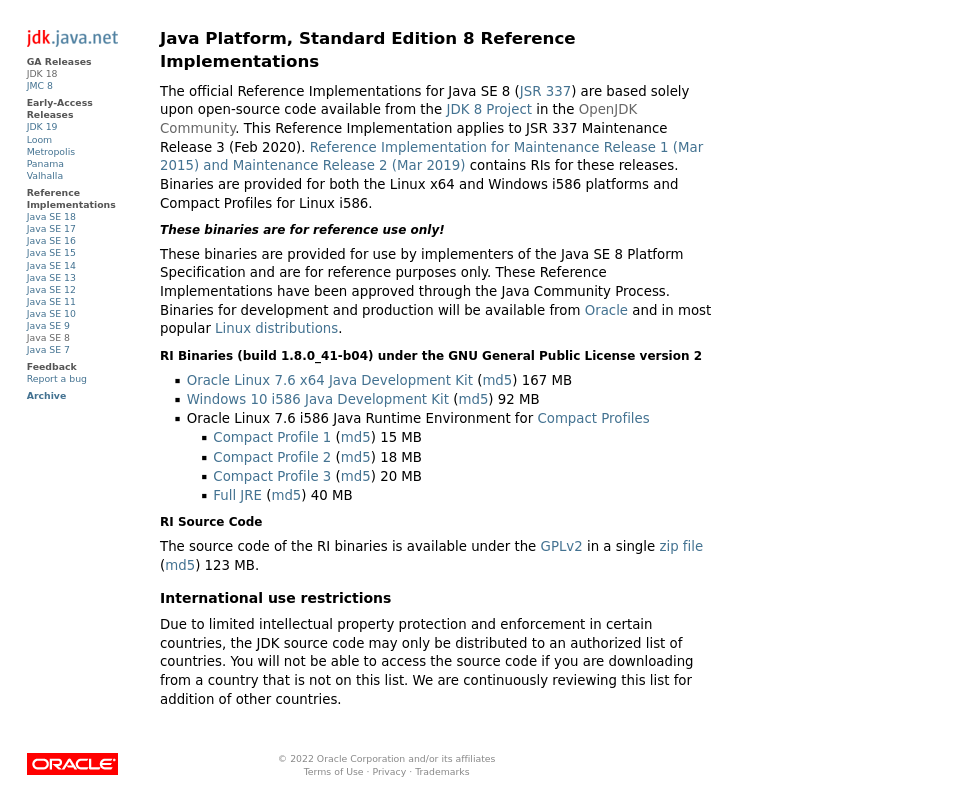
\includegraphics[height=6cm]{manual02}
  \end{subfigure}
  \caption{Capturas de los sitios web antes mencionados}
\end{figure}
Para los sistemas GNU/Linux, es muy probable que los repositorios de paquetes de muchísimas distribuciones ya tengan precompilados los correspondientes a varias versiones de Java, entre ellas, la 8, por ser una versión de largo plazo, y solo sería cosa de descargarlo usando el gestor de paquetes propio de cada distribución, y si no, siempre se puede encontrar el código fuente listo para compilar desde el sitio web de OpenJDK mostrado anteriormente.

\subsection{Ejecución}
En un sistema Windows, bastará con abrir el archivo \mintinline{bash}{programa.jar}. Se abrirá una consola, desde la cual operará el programa. En los sistemas GNU/Linux, sin embargo, esto no funcionará, ya que lo más probable es que este archivo no esté marcado como ejecutable, y no haya una asociación entre el tipo de archivo Jar, y el ejecutable del sistema Java. En este caso, será necesario abrir una consola en el directorio donde se encuentra el archivo Jar, y escribir el comando \mintinline{bash}{java -jar programa.jar}.
\begin{figure}
  \centering
  
\includegraphics[height=4cm]{manual03}
  \caption{Ícono probable del archivo Jar, en rojo}
  \label{fig:m3}
\end{figure}

\subsection{Primer inicio y sesión}
Al ejecutar el programa, lo primero que hace es comprobar si existe un archivo de sesión llamado \mintinline{bash}{datos.dat}, como se muestra en la figura \ref{fig:m3}, si existe, cargará los datos y la sesión que estuviese activa en el momento del guardado del archivo, si no, el programa avisará del hecho, y le invitará a crear una nueva cuenta de administrador para poder usar el programa, como se ve en la figura \ref{fig:m4}.

\begin{figure}
  \centering
  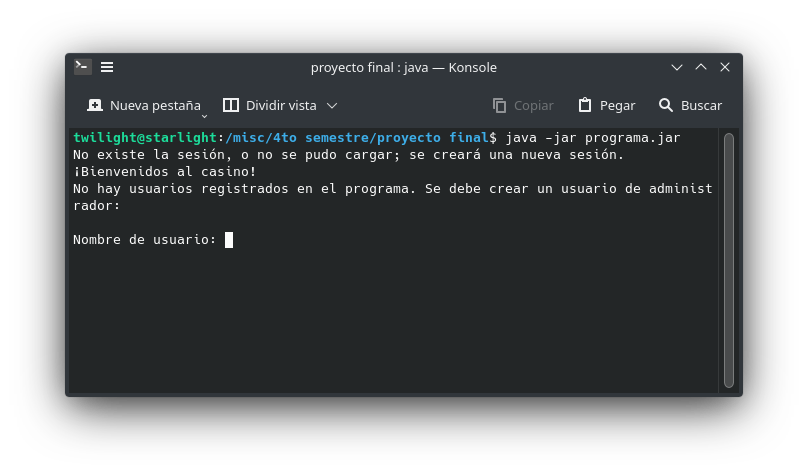
\includegraphics[height=8cm]{manual04}
  \caption{Creación del usuario administrador}
  \vspace{-1.5cm}
  \label{fig:m4}
\end{figure}

Una vez introducido un nombre de usuario, y una contraseña adecuada (ver \emph{Contraseña} en el glosario), el programa iniciará sesión automáticamente en la cuenta recién creada, y mostrará el menú de administrador. Esto le permitirá agregar todos los usuarios necesarios que usarán el programa, como se ve en la figura \ref{fig:m5}. Este procedimiento, y todo lo demás que un administrador puede realizar, se detalla en la sección \ref{admin}.
\begin{figure}
  \centering
  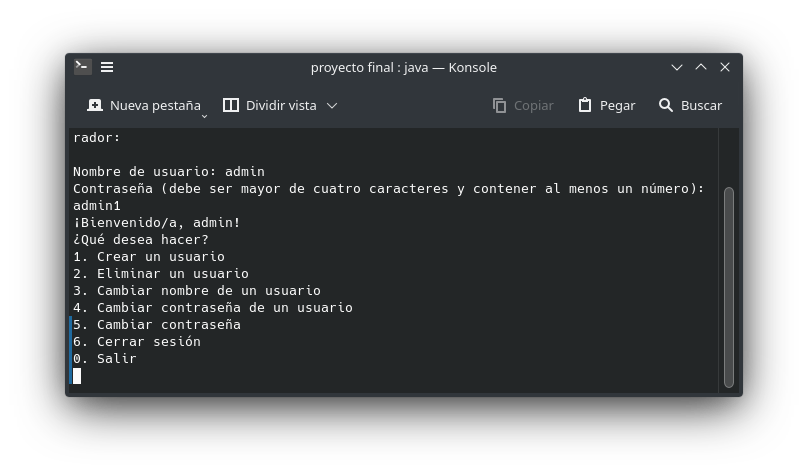
\includegraphics[height=8cm]{manual05}
  \vspace{-1.5cm}
  \caption{Menú de administrador}
  \label{fig:m5}
\end{figure}

Después de haber realizado todos los ajustes iniciales, en el menú, introducimon el valor 6, para terminar la sesión de administrador y poder iniciar sesión como jugador (ver figura \ref{fig:m6}). Ahora sí, el programa está listo para ser jugado, solo hace falta iniciar sesión en una cuenta de jugador, colocando el nommbre de usuario, y luego la contraseña. Si ambos datos son correctos, se mostrará el menú del usuario. Se ha de notar que se tiene 3 intentos para iniciar sesión correctamente: si se fallan los tres, el programa finalizará.

\begin{figure}
  \centering
  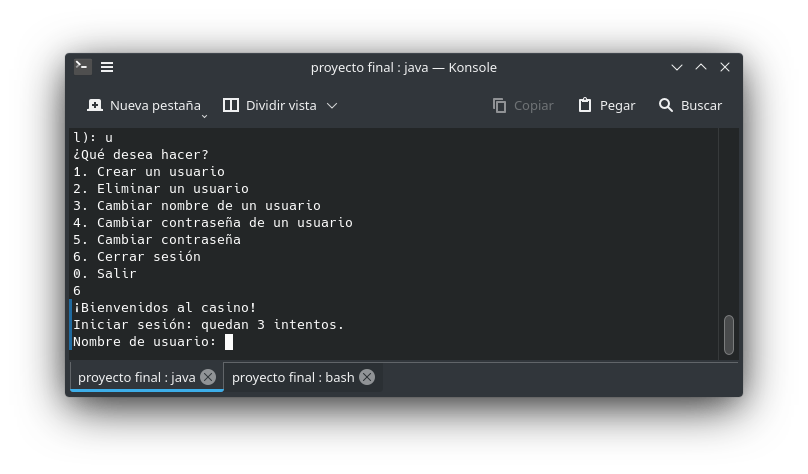
\includegraphics[height=8cm]{manual06}
  \vspace{-1.5cm}
  \caption{Primer inicio de sesión}
  \label{fig:m6}
\end{figure}
\begin{figure}
  \centering
  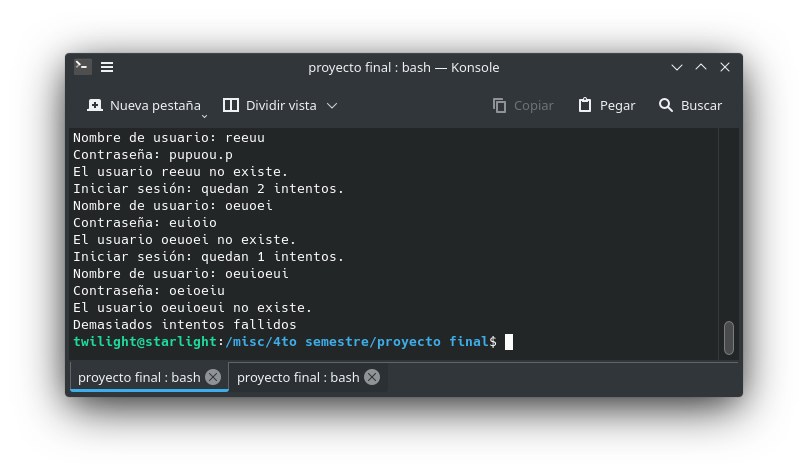
\includegraphics[height=8cm]{manual07}
  \vspace{-1.5cm}
  \caption{Demasiados intentos fallidos}
  \label{fig:m7}
\end{figure}

\section{Menú de jugador}
\label{jugador}
Una vez se ha iniciado sesión como jugador, se nos presentan 7 acciones posibles a realizar, como se ve en la figura \ref{fig:m8}. En la pantalla, también nos mostrará el número de créditos disponibles, y su equivalencia en pesos:

\begin{figure}
  \centering
  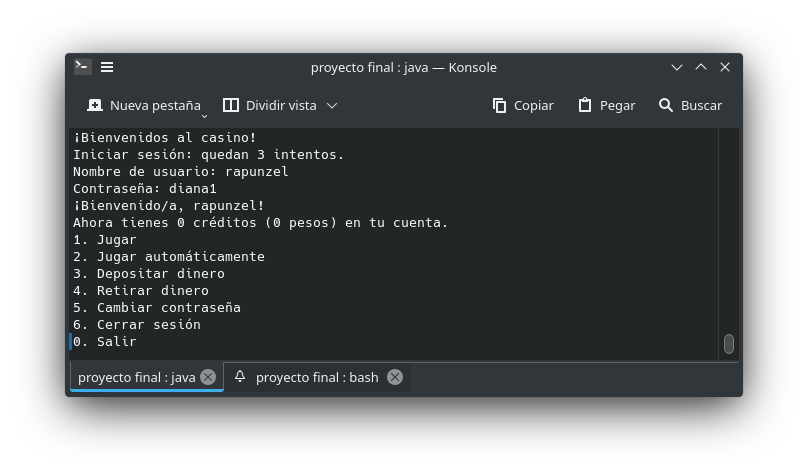
\includegraphics[height=8cm]{manual08}
  \vspace{-1.5cm}
  \caption{Menú de usuario}
  \label{fig:m8}
\end{figure}

\begin{description}[style=nextline]
\item[Jugar (1)]
  Permite jugar una ronda del tragamonedas
\item[Jugar automáticamente (2)]
  Permite jugar varias rondas del tragamonedas automáticamente
\item[Depositar dinero (3)]
  Permite comprar créditos para apostar
\item[Retirar dinero (4)]
  Permite retirar créditos, y convertirlos a pesos
\item[Cambiar contraseña (5)]
  Permite cambiar la contraseña del usuario
\item[Cerrar sesión (6)]
  Cierra la sesión para que otro usuario pueda jugar
\item[Salir (0)]
  Guarda el estado del programa y cierra el programa
\end{description}

\subsection{Jugar}
Esta opción nos permitirá jugar una ronda de la máquina tragamonedas. Se debe comprobar que tengamos créditos suficientes para la cantidad de dinero que deseemos apostar, si no es así, deberemos depositar dinero antes de empezar a jugar (ver sección \ref{deposito}).

Al seleccionar esta opción, el programa preguntará por la cantidad de dinero a apostar. Si se dispone del número de créditos necesarios, el juego «girará» aleatoriamente la máquina tragamonedas, mostrando el resultado de las combinaciones en pantalla, mediante una serie de letras (detallado en el glosario). Si hubo combinaciones ganadoras, se muestra la ganancia total en pesos. Las ganancias exactas se muestran en detalle en el Glosario.

\begin{figure}
  \centering
  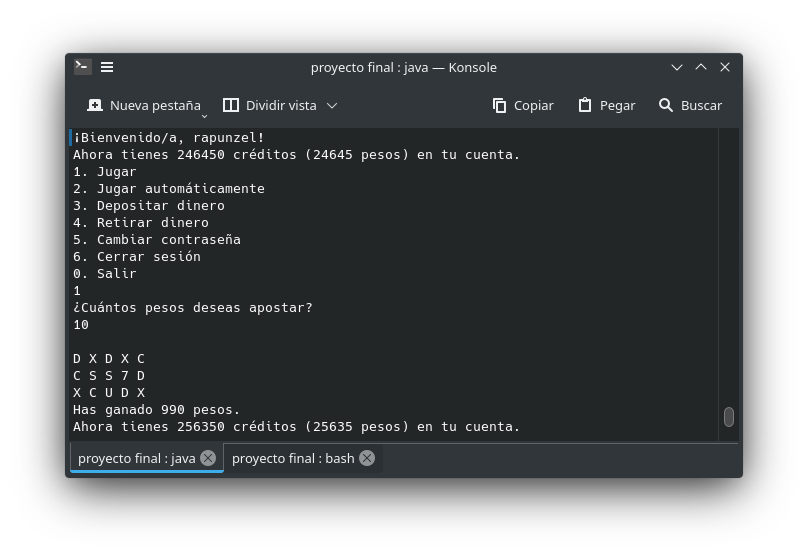
\includegraphics[height=8cm]{manual09}
  \vspace{-1cm}
  \caption{Jugar}
  \label{fig:m9}
\end{figure}

La figura \ref{fig:m9} muestra como un usuario tenía 24645 pesos, apostó 10, y ganó 1000 pesos (porque una combinación de cuatro diamantes vale 1000 pesos), menos los 10 pesos iniciales de apuesta, quedando con 25635 pesos.

\subsection{Jugar automáticamente}
Esta opción es similar a la anterior, pero, además, el programa preguntará cuántas veces se desea repetir el juego. El juego, entonces, mostrará el progreso de cada juego, cuándo se gana (o pierde) en cada uno, y cuánto se ganó (o perdió) en total. Por ejemplo, en la figura \ref{fig:m10} se muestra cómo se apostó tres veces 10 pesos, perdiéndose todas las jugadas, y perdiendo al final 30 pesos.

\begin{figure}
  \centering
  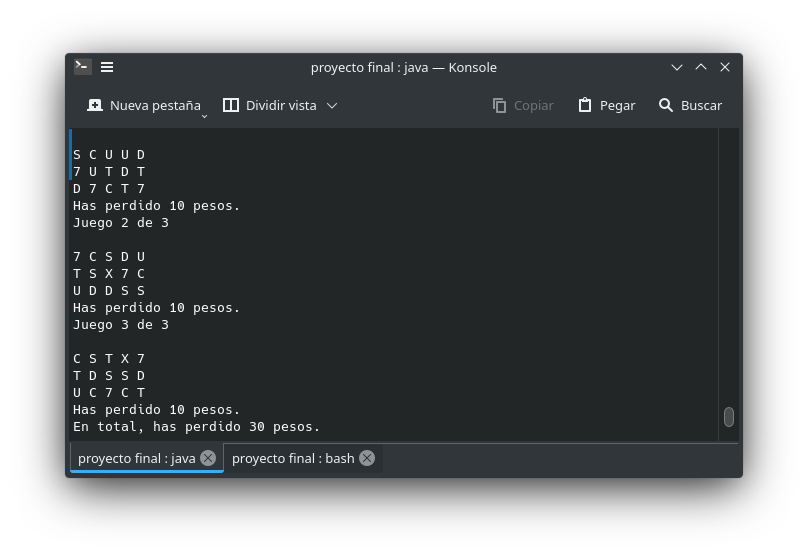
\includegraphics[height=8cm]{manual10}
  \vspace{-1cm}
  \caption{Jugar automáticamente}
  \label{fig:m10}
\end{figure}

\subsection{Depositar dinero}
\label{deposito}
Esta opción te permite depositar dinero en la cuenta del usuario. Este dinero será convertido a créditos, de modo que lo que termina almacenándose en la cuenta son los créditos. Para saber más sobre los créditos, léase la entrada en el glosario.

Al seleccionar esta opción, se preguntará cuántos pesos desea gastar para conseguir créditos. La cantidad mínima es de 20 pesos, es decir, como mínimo se pueden adquirir 200 créditos. Por otra parte, la mayor cantidad que se puede poseer en una cuenta es de un millón de pesos, o 10 millones de créditos, por lo que cualquier intento de ingresar dinero para tener una mayor cantidad fallará. En la figura \ref{fig:m11} se puede observar cómo después de poseer 0 créditos, se adquirieron 10000 pagando mil pesos por ellos.
\begin{figure}
  \centering
  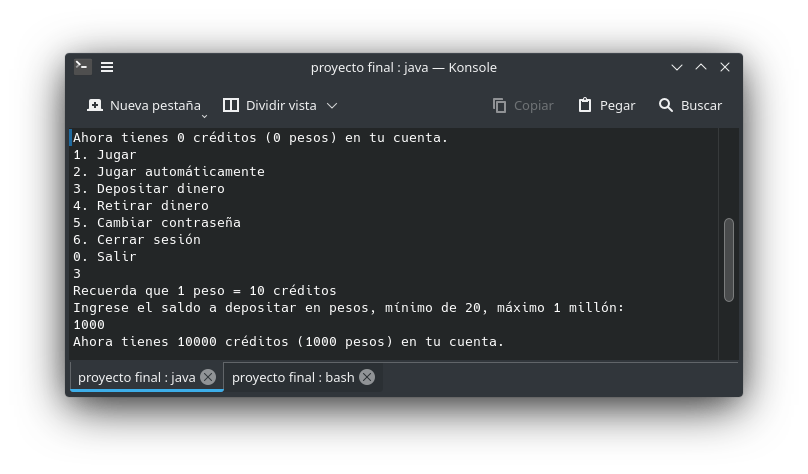
\includegraphics[height=8cm]{manual11}
  \vspace{-1.5cm}
  \caption{Depositar dinero}
  \label{fig:m11}
\end{figure}

\subsection{Retirar dinero}
Así como se puede ingresar dinero, esta opción te permitirá cambiar créditos por dinero, retirándolo. Al seleccionar esta opción, el programa preguntará cuánto dinero deseas retirar, con la única limitante de no poder retirar más dinero del que pueda comprarse con los créditos que se poseen. En la figura \ref{fig:m12} se puede observar cómo después de poseer 1000 créditos, se retiraron la mitad pagando 500 pesos por ellos.
\begin{figure}
  \centering
  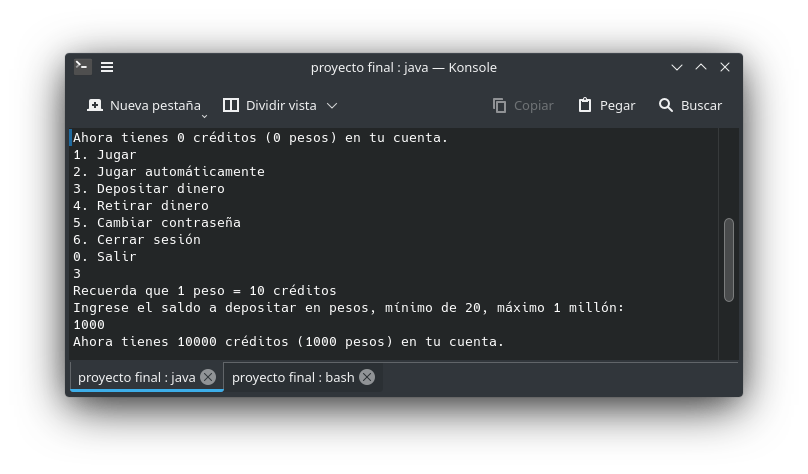
\includegraphics[height=8cm]{manual12}
  \vspace{-1.5cm}
  \caption{Retirar dinero}
  \label{fig:m12}
\end{figure}

\subsection{Cambiar contraseña}
\label{contra}
Esta opción permite cambiar la contraseña del usuario que tiene la sesión activa (figura \ref{fig:m13}). Al seleccionar esta opción, el programa preguntará por la contraseña actual, para asegurarse de que el usuario realmente desea cambiar la contraseña; y luego, preguntará la nueva contraseña. La nueva contraseña deberá también cumplir los requisitos de seguridad, de lo contrario, la operación fallará.
\begin{figure}
  \centering
  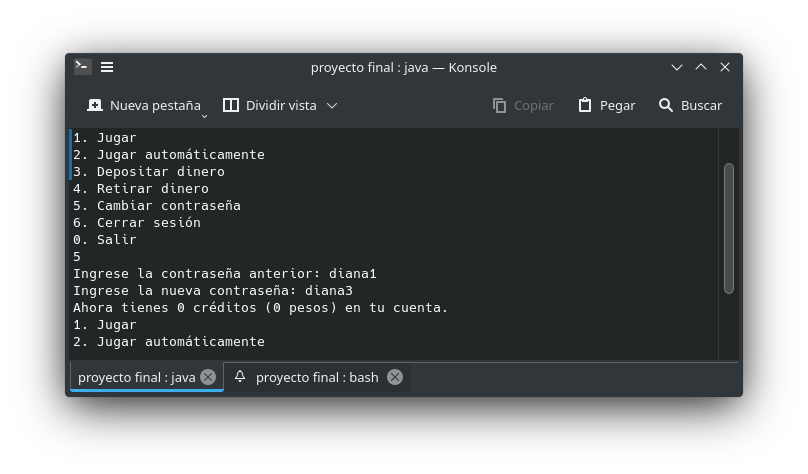
\includegraphics[height=8cm]{manual13}
  \vspace{-1.5cm}
  \caption{Cambiar contraseña}
  \label{fig:m13}
\end{figure}

\subsection{Cerrar sesión}
\label{cerrar}
Esta opción cierra la sesión del usuario, permitiendo a otro usuario jugar. Después de seleccionar esta opción, se mostrará la pantalla para iniciar sesión nuevamente.
\subsection{Salir}
\label{salir}
Esta opción simplemente cierra el juego y guarda el estado del programa.

\section{Menú de administrador}
\label{admin}
Cuando se inicia una sesión como administrador, no muestra elementos para jugar. En su lugar, tenemos 7 acciones posibles, como se ve en la figura \ref{fig:m4}, encaminadas a la administración de otros usuarios.

\begin{description}[style=nextline]
\item[Crear un usuario (1)]
  Permite añadir usuarios nuevos al programa
\item[Eliminar un usuario (2)]
  Permite quitar usuarios del programa
\item[Cambiar nombre de un usuario (3)]
  Permite cambiar el nombre de cualquier usuario del programa
\item[Cambiar contraseña de un usuario (4)]
  Permite cambiar la contraseña de cualquier usuario del programa
\item[Cambiar contraseña (5)]
  Permite cambiar la contraseña del usuario
\item[Listar usuarios (6)]
  Permite listar todos los usuarios en el programa
\item[Cerrar sesión (7)]
  Cierra la sesión para que otro usuario pueda jugar
\item[Salir (0)]
  Guarda el estado del programa y cierra el programa
\end{description}

\subsection{Crear un usuario}
Esta opción permite al administrador agregar al programa nuevos usuarios, sean jugadores o administradores. Al seleccionarla, preguntará primero el nombre del usuario, que no debe existir ya en el programa. Luego, pedirá una contraseña, que debe cumplir con los requisitos de seguridad; y finalmente, preguntará si la cuenta será de tipo administrador o jugador. Se ha de escribir una «a» si es del primer tipo, y cualquier otro caracter en el otro caso. En la figura \ref{fig:m14} se creó un usuario nuevo, con el nombre \emph{rapunzel}, con contraseña \emph{diana1}, y de tipo jugador. Los detalles sobre el nombre de usuario se indican en el glosario.

\begin{figure}
  \centering
  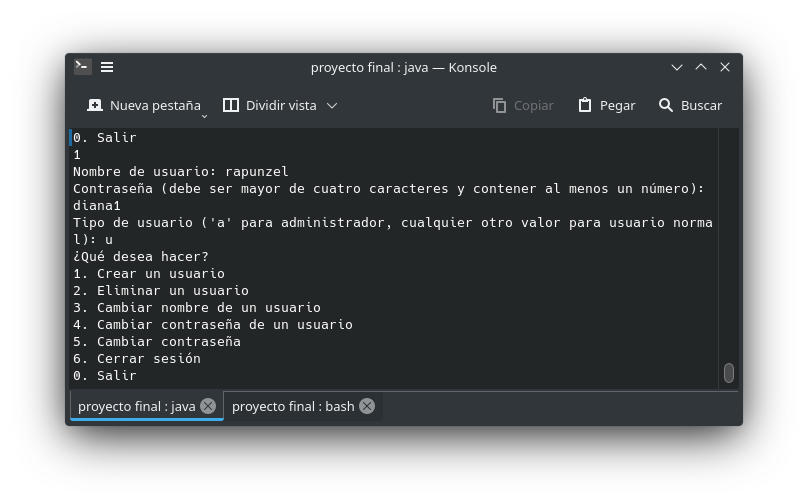
\includegraphics[height=8cm]{manual14}
  \vspace{-1cm}
  \caption{Crear un usuario}
  \label{fig:m14}
\end{figure}

\subsection{Eliminar un usuario}
Esta opción permite al administrador eliminar del programa usuarios existentes, de manera que ya no estén disponibles. Al seleccionarla, preguntará solamente el nombre del usuario a eliminar, que debe existir, de lo contrario, generará un error. En la figura \ref{fig:m15} se muestra cómo se eliminó un usuario de nombre \emph{asdfg}.

\begin{figure}
  \centering
  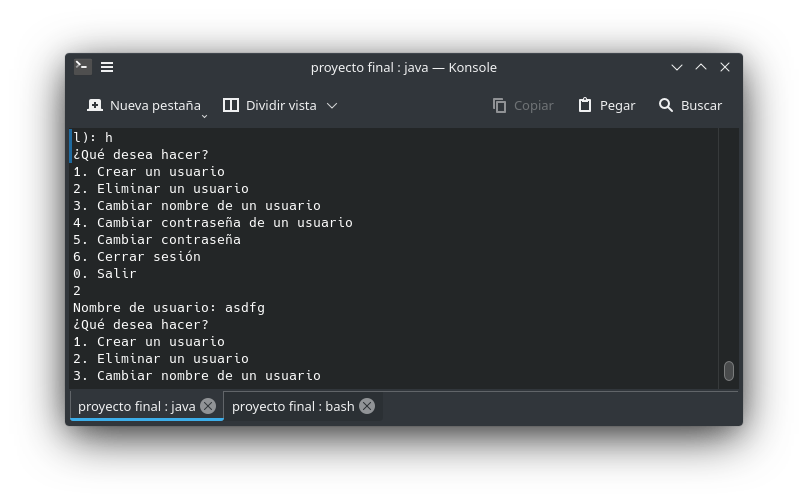
\includegraphics[height=8cm]{manual15}
  \vspace{-1cm}
  \caption{Eliminar un usuario}
  \label{fig:m15}
\end{figure}

\subsection{Cambiar nombre de un usuario}
Esta opción permite al administrador cambiar el nombre de un usuario por otro. Al seleccionarla, el programa preguntará el nombre del usuario a renombrar, que debe existir; y luego, preguntará por el nuevo nombre, que no debe pertenecer ya a otro usuario existente. En la figura \ref{fig:m16} se muestra cómo se cambió el nombre del usuario \emph{rapunzel} al nombre \emph{cenicienta}.

\begin{figure}
  \centering
  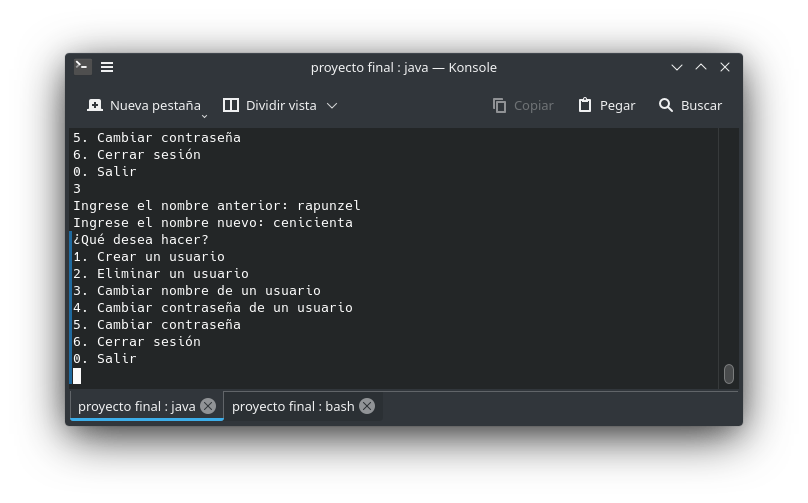
\includegraphics[height=8cm]{manual16}
  \vspace{-1cm}
  \caption{Cambiar nombre de un usuario}
  \label{fig:m16}
\end{figure}

\subsection{Cambiar contraseña de un usuario}
Esta opción permite al administrador cambiar la contraseña de un usuario cualquiera por otra, excepto la propia cuenta del administrador, cuyo procedimiento se detalla en la sección \ref{contra}. Al seleccionarla, el programa preguntará el nombre del usuario cuya contraseña se modificará, y luego preguntará por la contraseña nueva (contrasta con el modo de cambiar la contraseña propia, que además, pide una confirmación mediante la contraseña actual). En la figura \ref{fig:m17} se muestra cómo se reemplazó la contraseña del usuario \emph{cenicienta} por la contraseña \emph{diana33}.

\begin{figure}
  \centering
  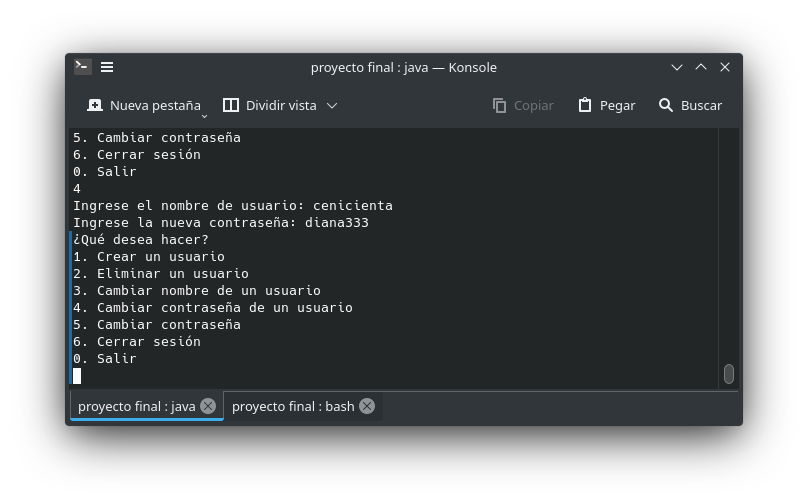
\includegraphics[height=8cm]{manual17}
  \vspace{-1cm}
  \caption{Cambiar contraseña de un usuario}
  \label{fig:m17}
\end{figure}

\subsection{Cambiar contraseña}
Véase la sección \ref{contra}.

\subsection{Listar usuarios}
Esta opción permite listar todos los usuarios existentes en el programa. Al seleccionar esta opción, simplemente se mostrarán los nombres de los usuarios en línea, sin ningún detalle adicional. En la figura \ref{fig:m18}, se listan dos usuarios: \emph{admin} y \emph{cenicienta}.

\begin{figure}
  \centering
  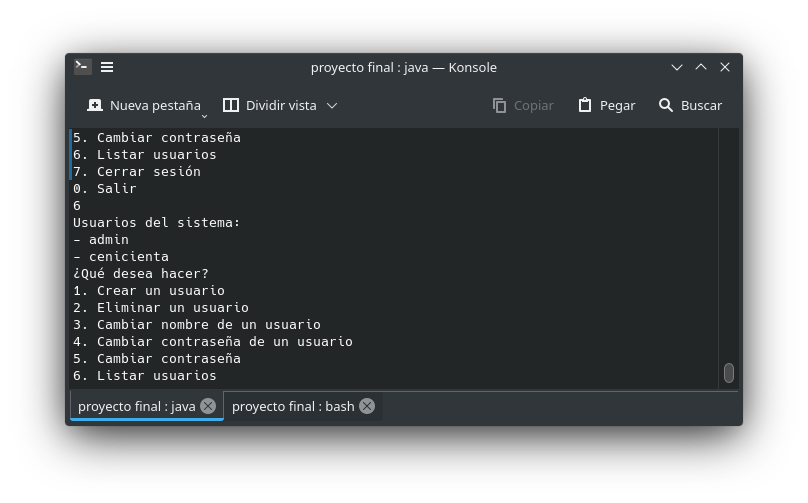
\includegraphics[height=8cm]{manual18}
  \vspace{-1cm}
  \caption{Listar usuarios}
  \label{fig:m18}
\end{figure}

\subsection{Cerrar sesión}
Véase la sección \ref{cerrar}.

\subsection{Salir}
Véase la sección \ref{salir}.

\section{Glosario}
\begin{description}[style=nextline]
\item[Contraseña]
  Una contraseña es la forma que tiene un usuario de poder entrar a su cuenta, de manera que el programa esté seguro que solamente el usuario, y no otra persona, sea quien entra a su cuenta. Por lo tanto, para que una contraseña cumpla su función de seguridad, el programa establece unos requisitos básicos:
  \begin{itemize}
    \item{\textbf{La contraseña debe tener como mínimo cuatro caracteres.} Contraseñas más cortas serán rechazadas por el sistema.}
    \item{\textbf{La contraseña debe tener, al menos, un dígito}. Una contraseña de puras letras es muy fácil de adivinar.}
  \end{itemize}
\item[Crédito]
  Un crédito es la unidad básica de moneda dentro del juego. Mientras que el usuario piensa en pesos, dentro del juego, todos los precios de las apuestas y ganancias se contabilizan en créditos, convirtiéndose en pesos solamente cuando se interactúa con el usuario. Un crédito es equivalente a una décima de un peso.
\item[Nombre]
  El nombre de un usuario es una cadena de texto que identifica a la cuenta, entonces no puede haber dos cuentas con el mismo nombre. El programa no impone ninguna restricción en cuanto a los nombres, pero se recomienda que sean cortos, que los caracteres sean solo los pertenecientes a ASCII, y que no mezclen minúsculas con mayúsculas.
\item[Símbolo]
  En una máquina tragamonedas, un símbolo es cualquiera de las figuras que pueden salir en los rodillos de la máquina tragamonedas. En este juego, se consideran siete símbolos, mostrados en esta tabla, junto con sus representaciones Unicode y ASCII, y los créditos que otorgan cuando se hace una combinación con cierta cantidad de elementos:
  \begin{tabular}{ c | c c c c c }
    Símbolo & Car. Unicode & Car. ASCII & 3 comb. & 4 comb. & 5 comb. \\
    \hline
    Comodín & \emoji{game-die} & X & 15000 & 30000 & 100000 \\
    Siete & 7️ & 7 & 10000 & 25000 & 50000 \\
    Diamante & \emoji{gem-stone} & D & 2500 & 5000 & 10000 \\
    Trébol & \emoji{four-leaf-clover} & T & 650 & 1250 & 2500 \\
    Cereza & \emoji{cherries} & C & 600 & 1000 & 1500 \\
    Sandía & \emoji{watermelon} & S & 160 & 325 & 650 \\
    Uvas & \emoji{grapes} & U & 160 & 325 & 650
  \end{tabular}
\item[Usuario]
  Cualquier persona con una cuenta en el programa. Hay dos tipos de usuarios: \emph{administradores} y \emph{jugadores}.
\end{description}
\end{document}
